\documentclass{ximera}
\graphicspath{{./content/hw_03_parametrized_curves/graphics/}{./graphics/}}
\title{Homework 3: Parametrized Curves}
\begin{document}
\begin{abstract}
\end{abstract}
\maketitle
\section*{Online Problems}

\begin{problem}
Several parametrized curves are graphed below, and the arrow indicates the direction in which the parameter increases. Which is the graph of the path $\vec{x}(t) = (4-t, 2t+1)$, for $-1\leq t\leq 1$?
\begin{multipleChoice}
\choice{\begin{image}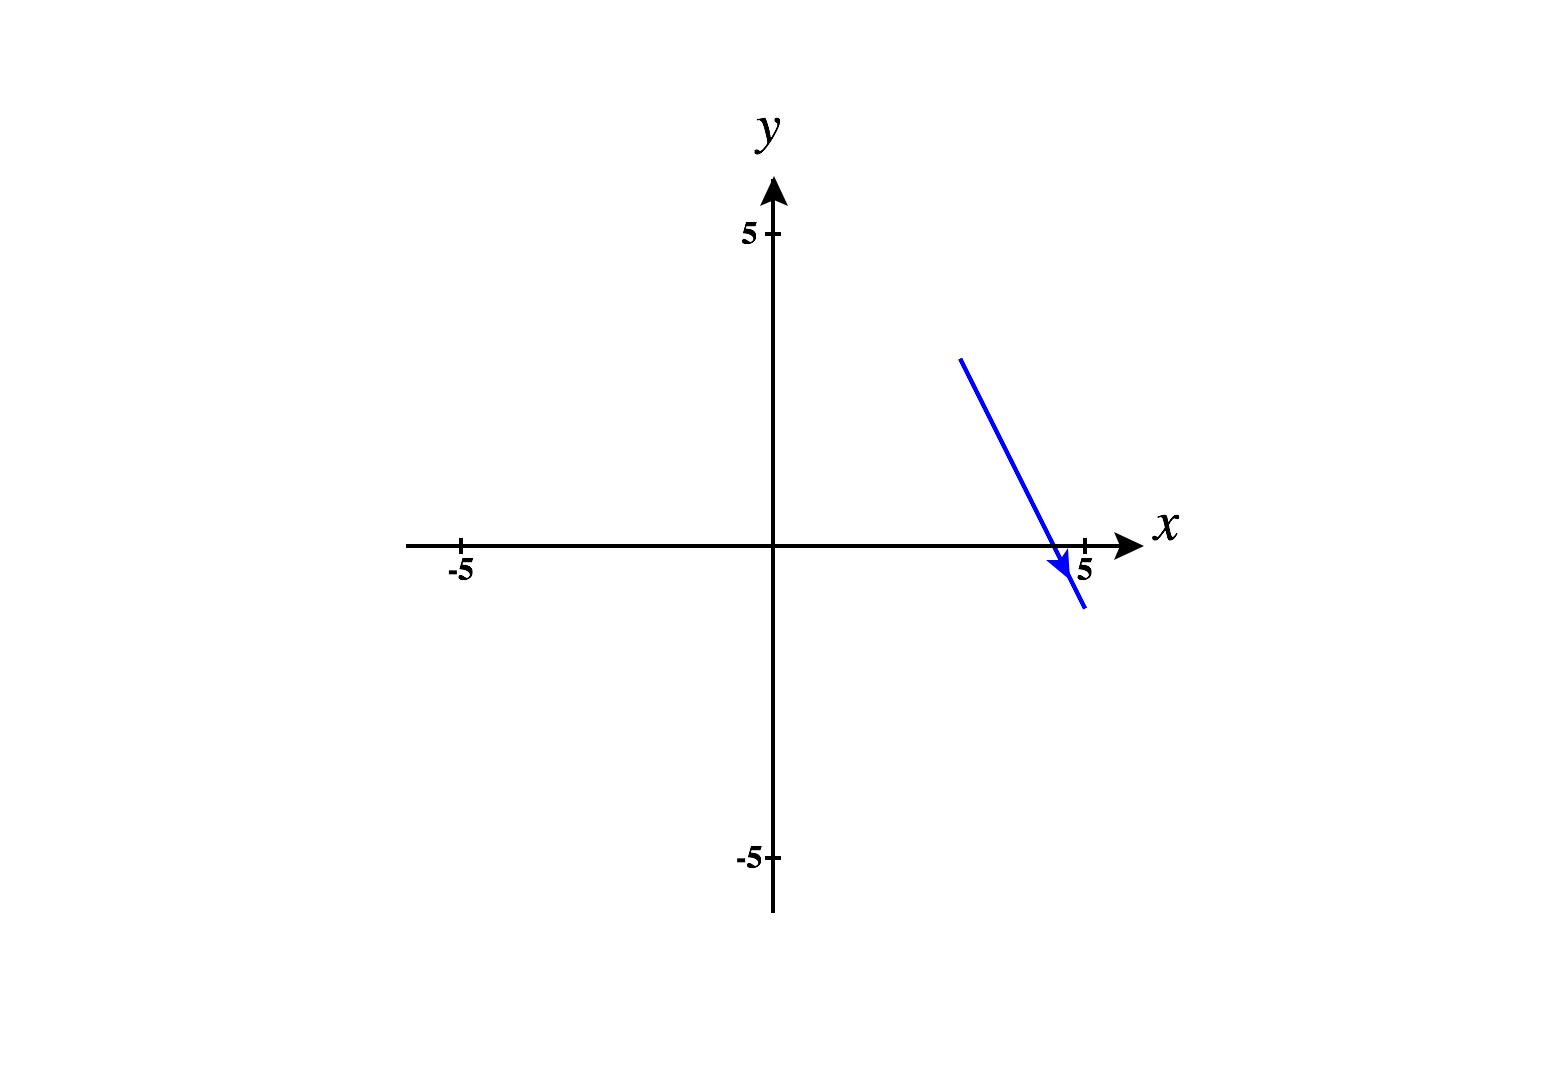
\includegraphics[width =\textwidth]{CalcPlot3D-line_incorrect1}\end{image}}
\choice[correct]{\begin{image}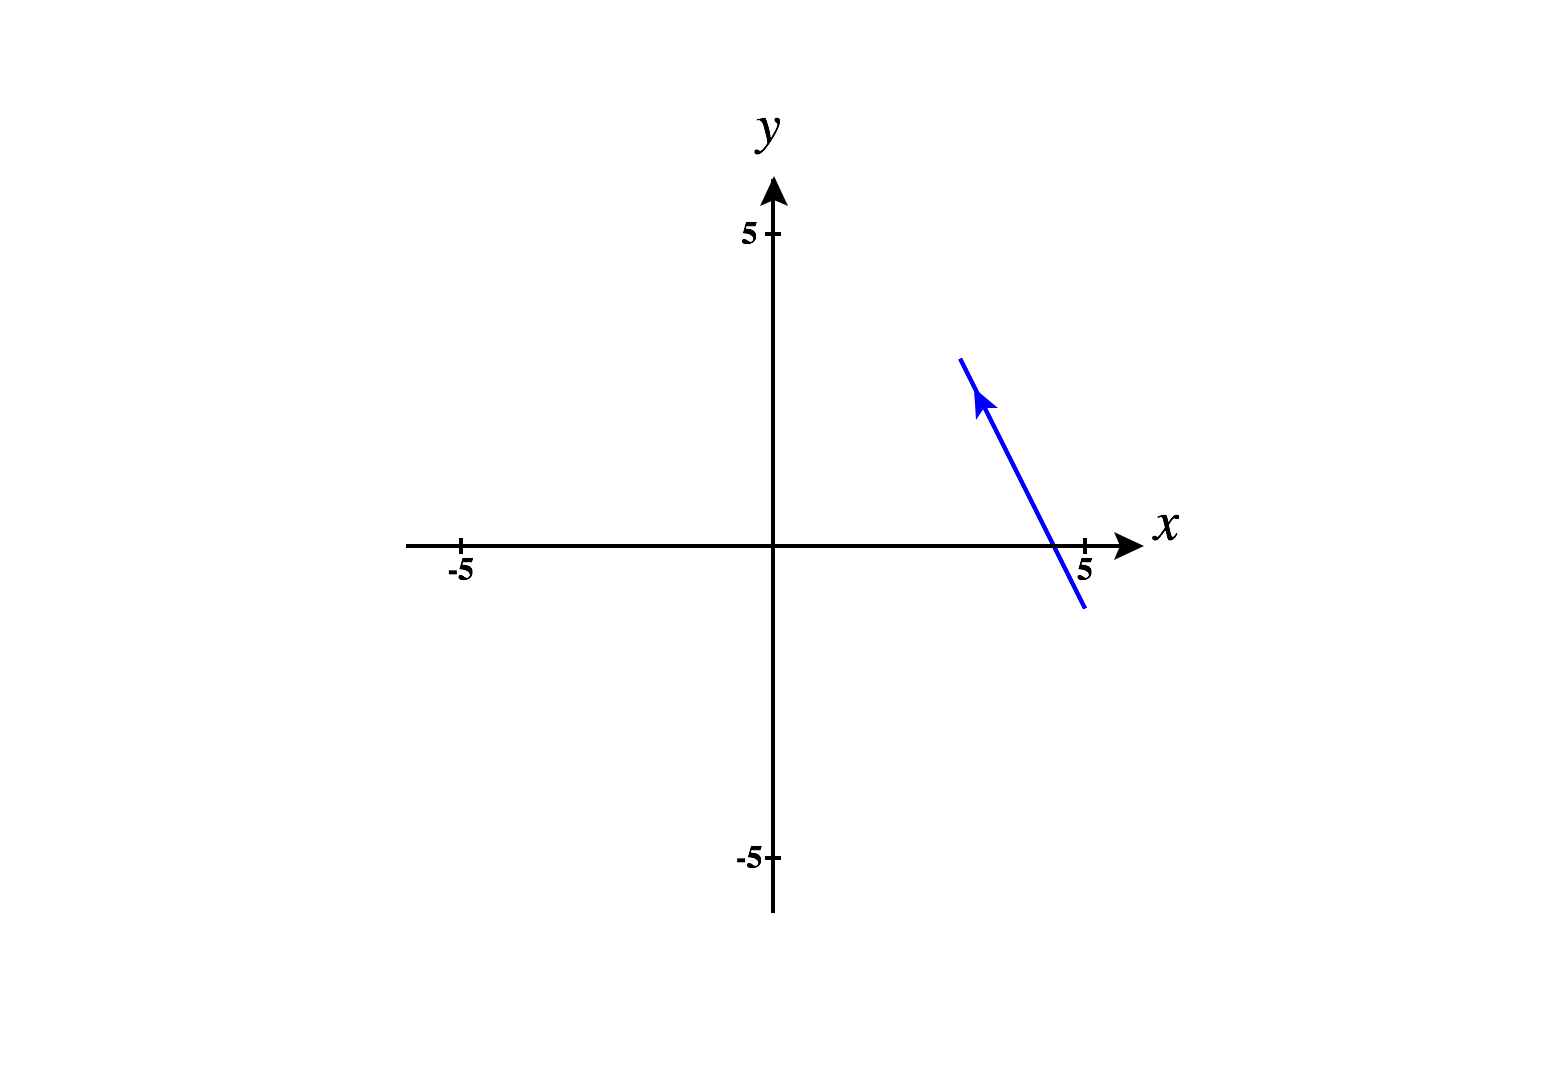
\includegraphics[width =\textwidth]{CalcPlot3D-line_correct}\end{image}}
\choice{\begin{image}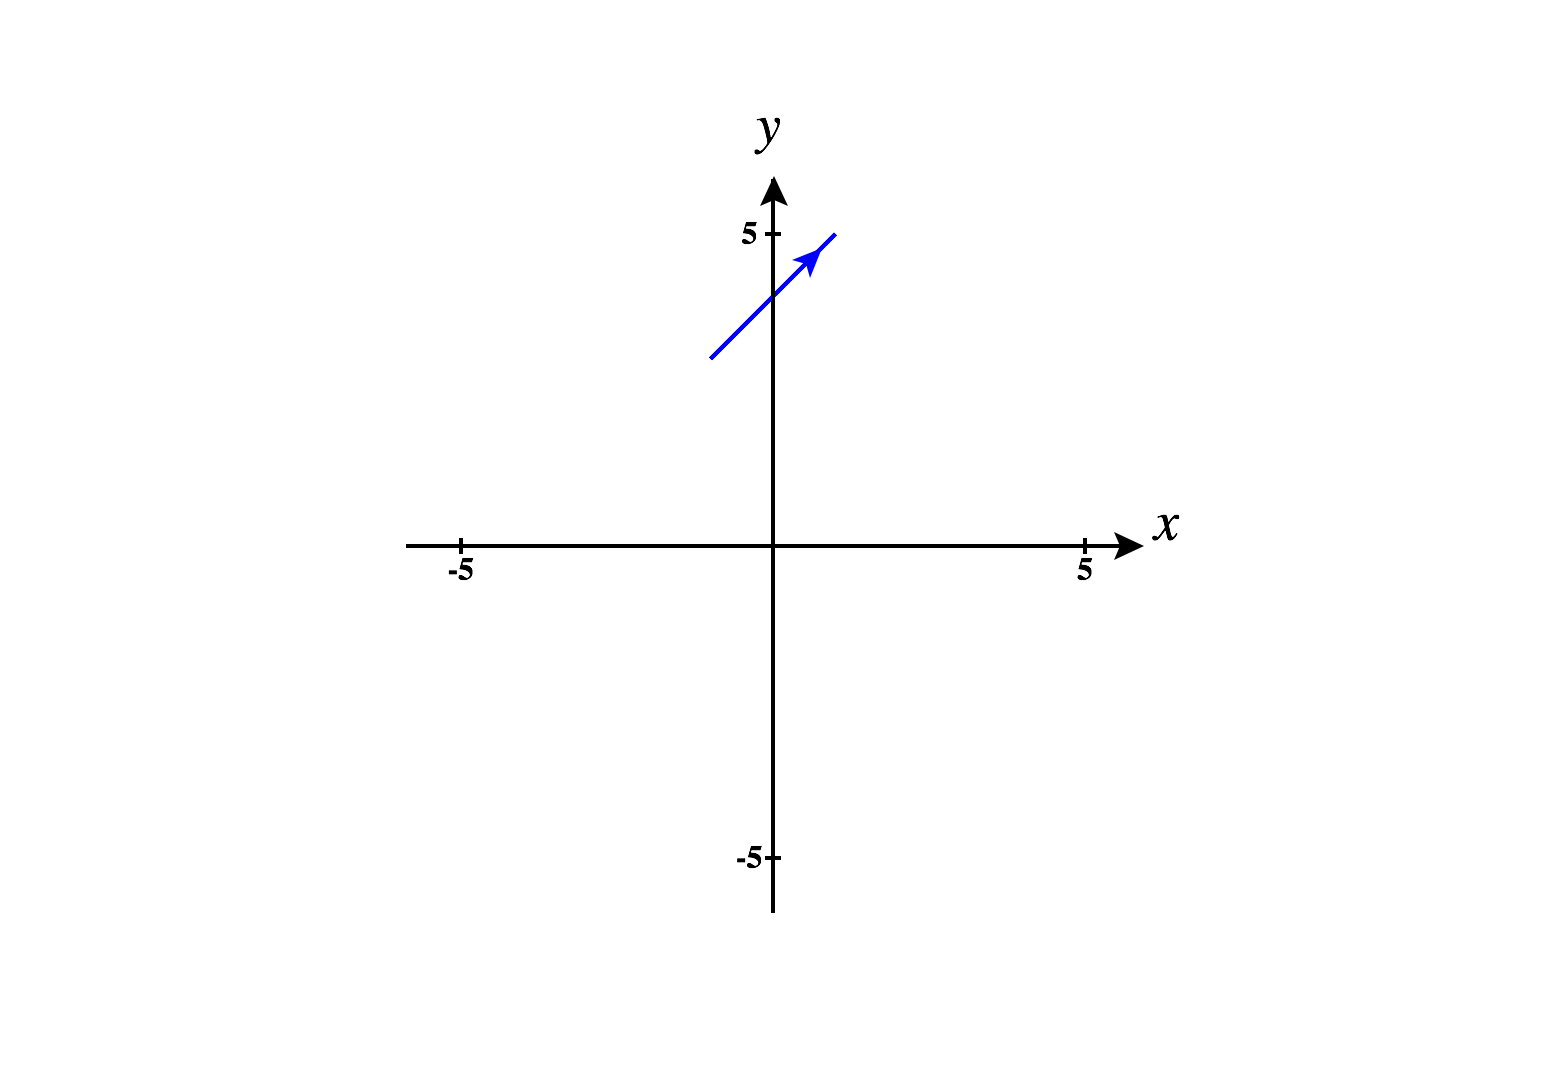
\includegraphics[width =\textwidth]{CalcPlot3D-line_incorrect2}\end{image}}
\choice{\begin{image}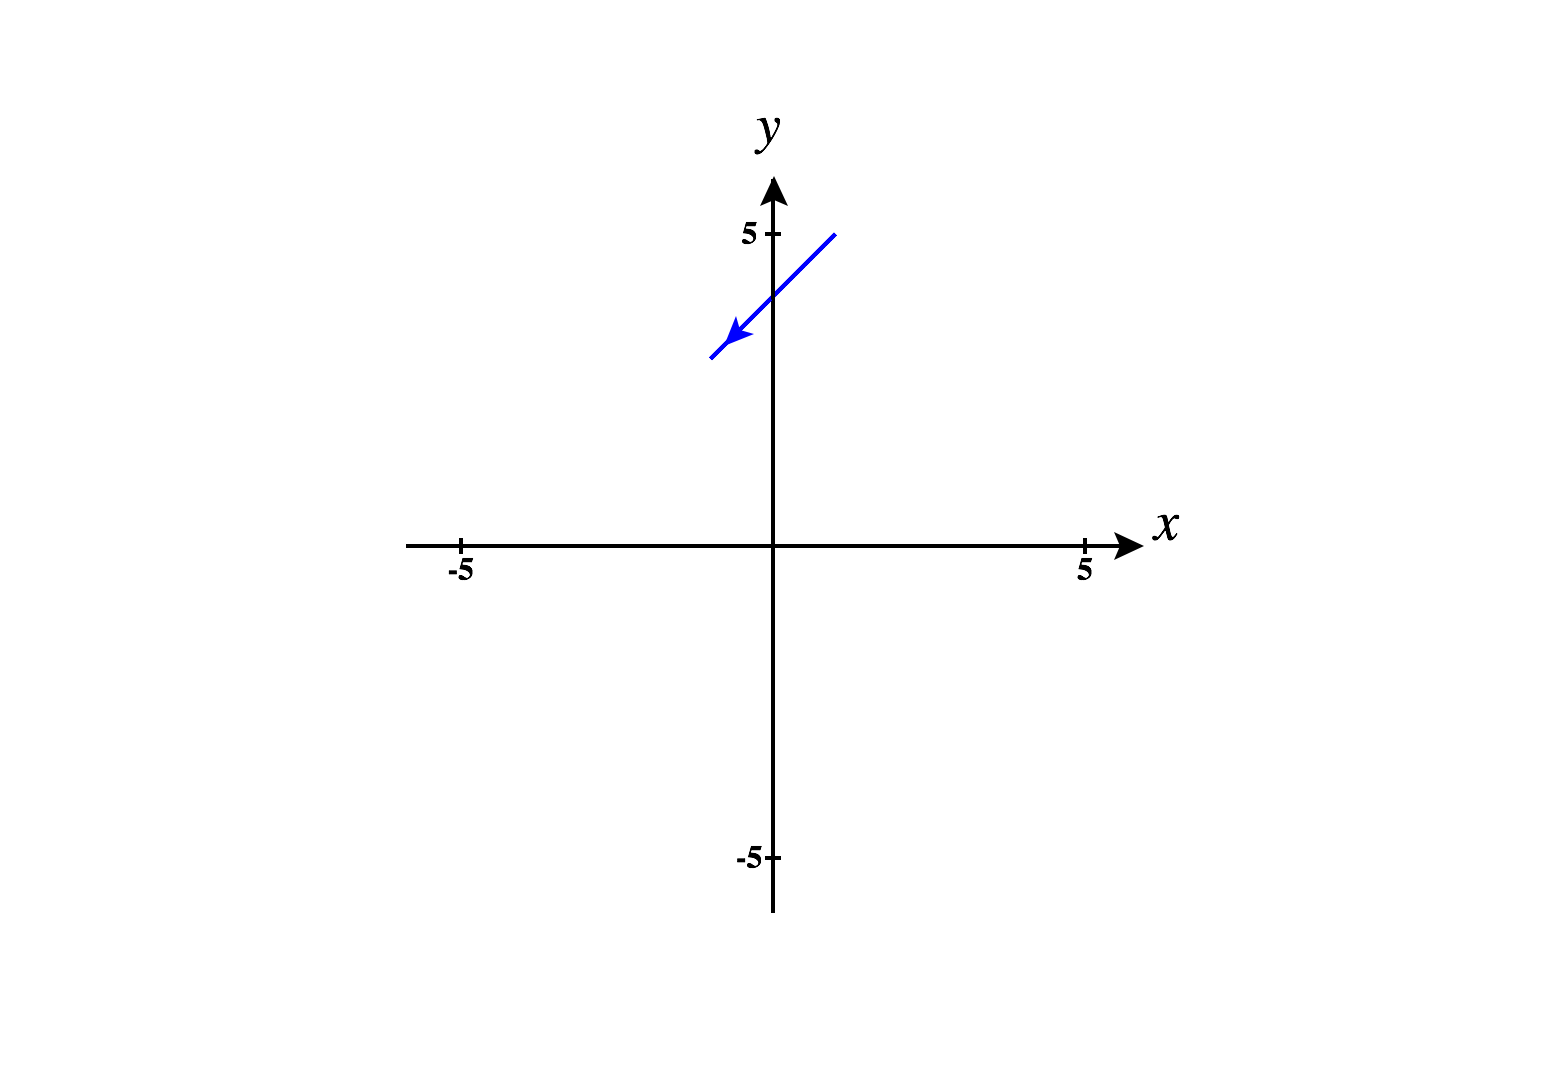
\includegraphics[width =\textwidth]{CalcPlot3D-line_incorrect3}\end{image}}
\choice{\begin{image}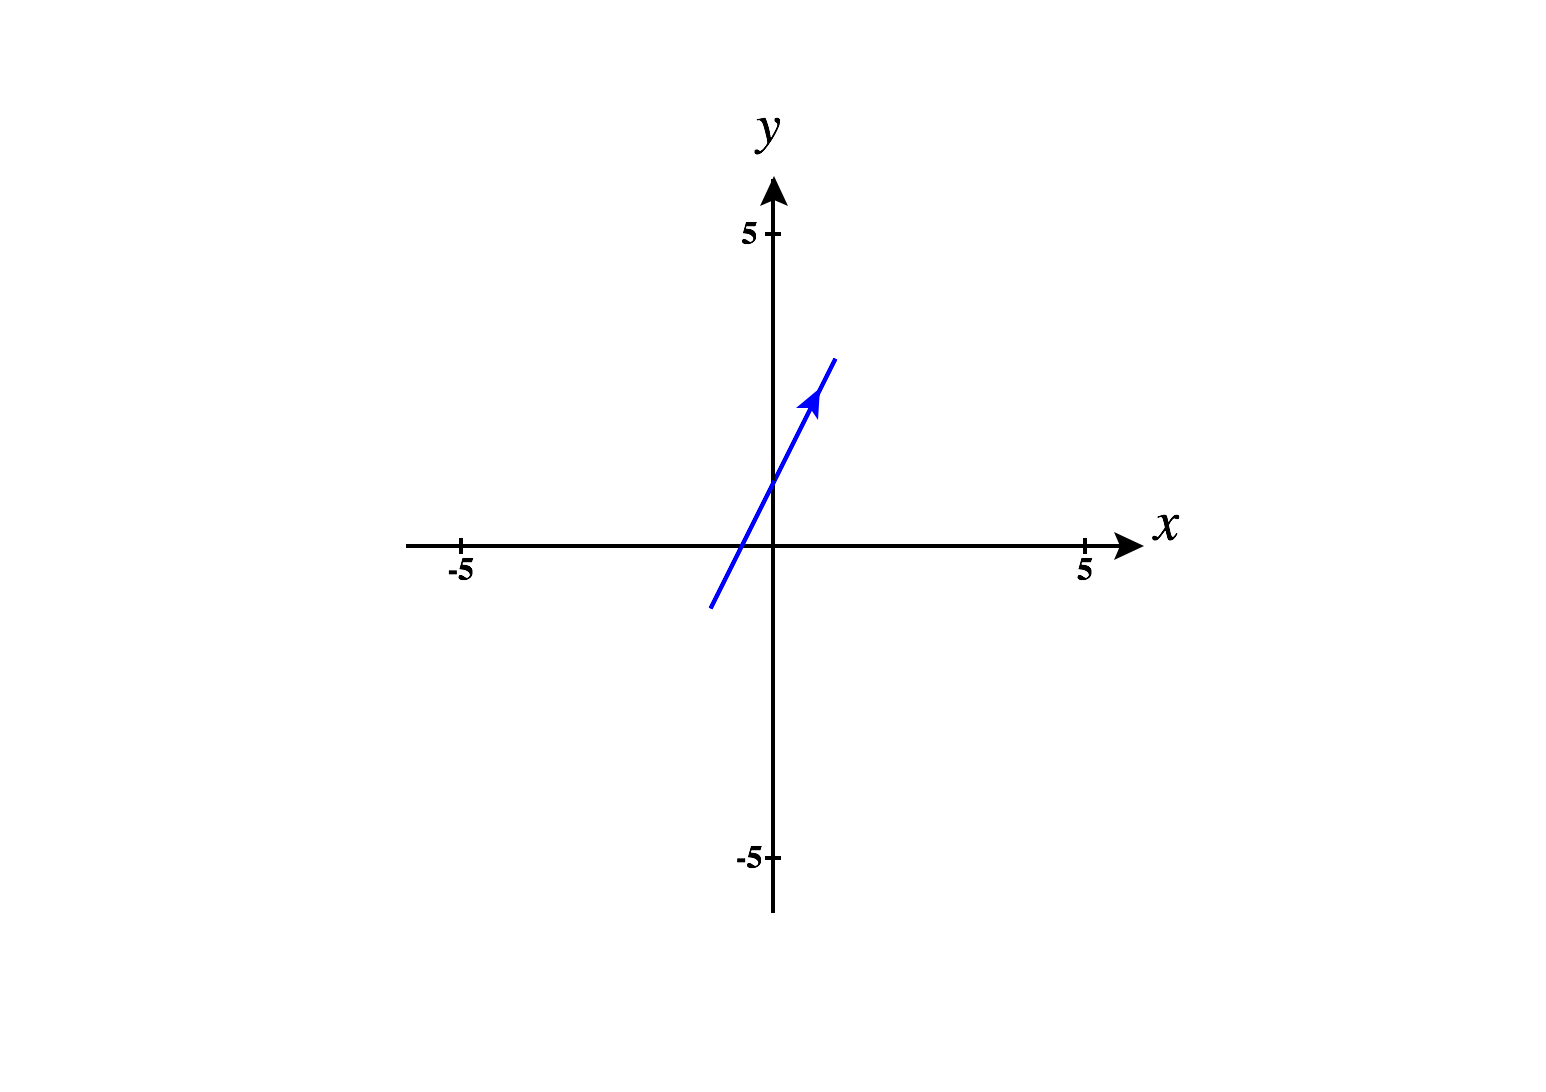
\includegraphics[width =\textwidth]{CalcPlot3D-line_incorrect4}\end{image}}
\choice{\begin{image}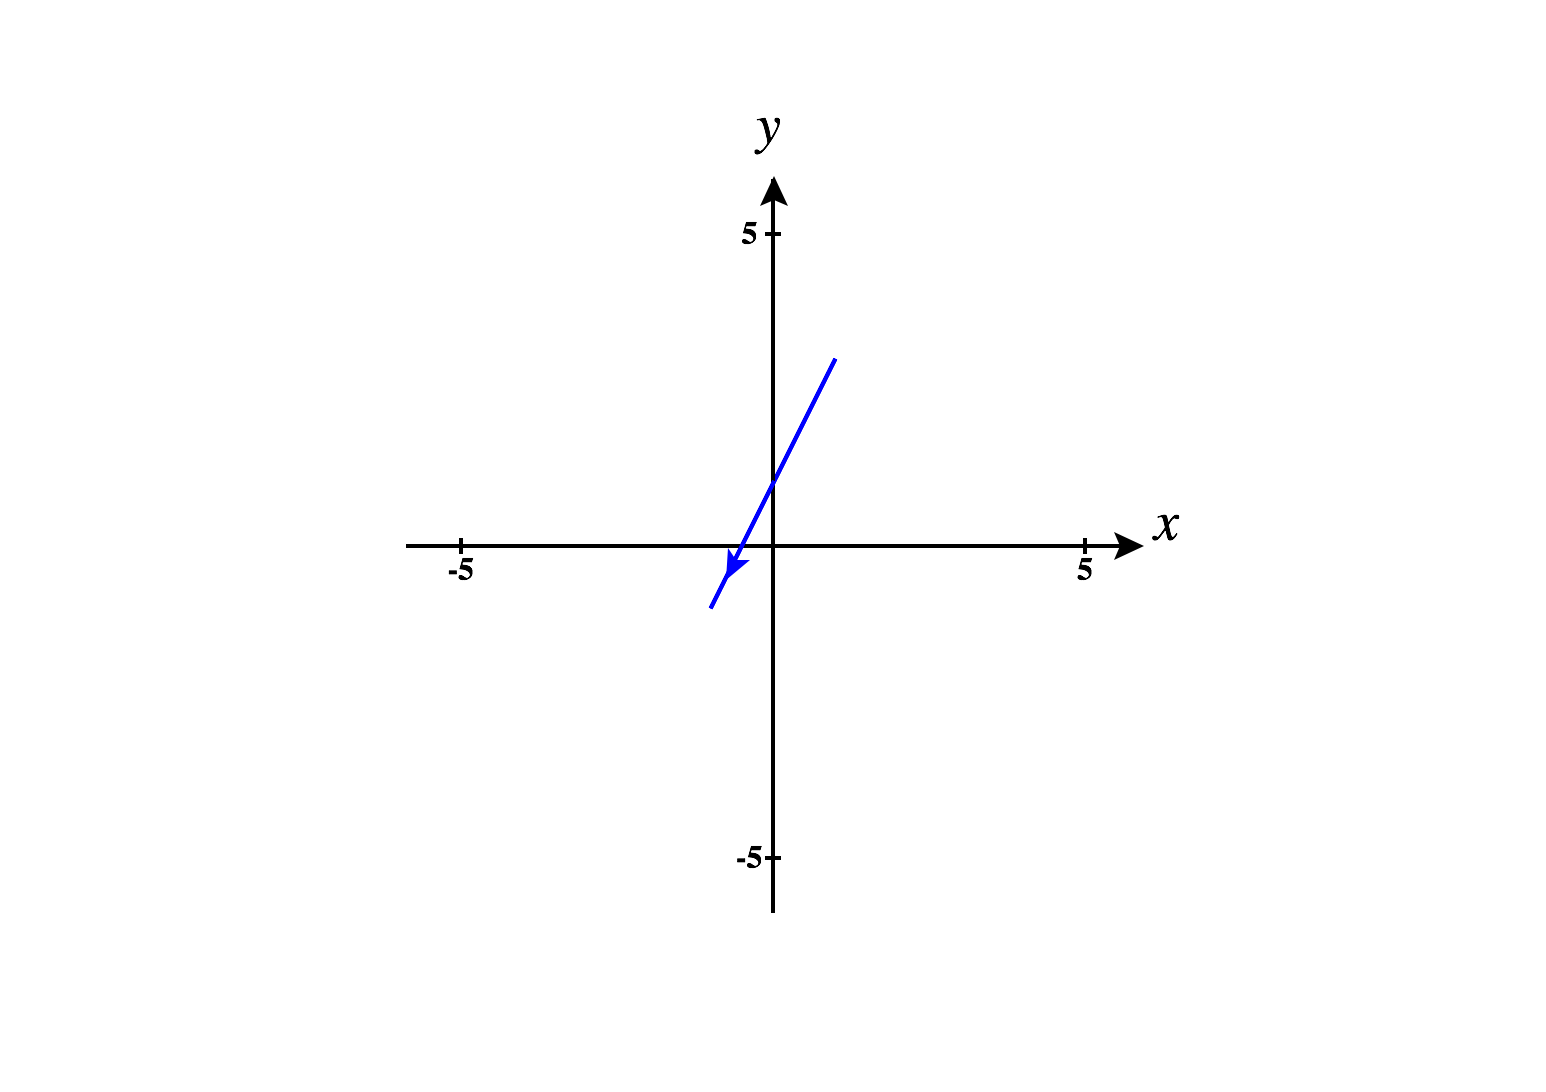
\includegraphics[width =\textwidth]{CalcPlot3D-line_incorrect5}\end{image}}
\end{multipleChoice}
\end{problem}

\begin{problem}
Several parametrized curves are graphed below, and the arrow indicates the direction in which the parameter increases. Which is the graph of the path $\vec{x}(t) = (t^2, t^3)$, for $-1\leq t\leq 1$?
\begin{multipleChoice}
\choice[correct]{\begin{image}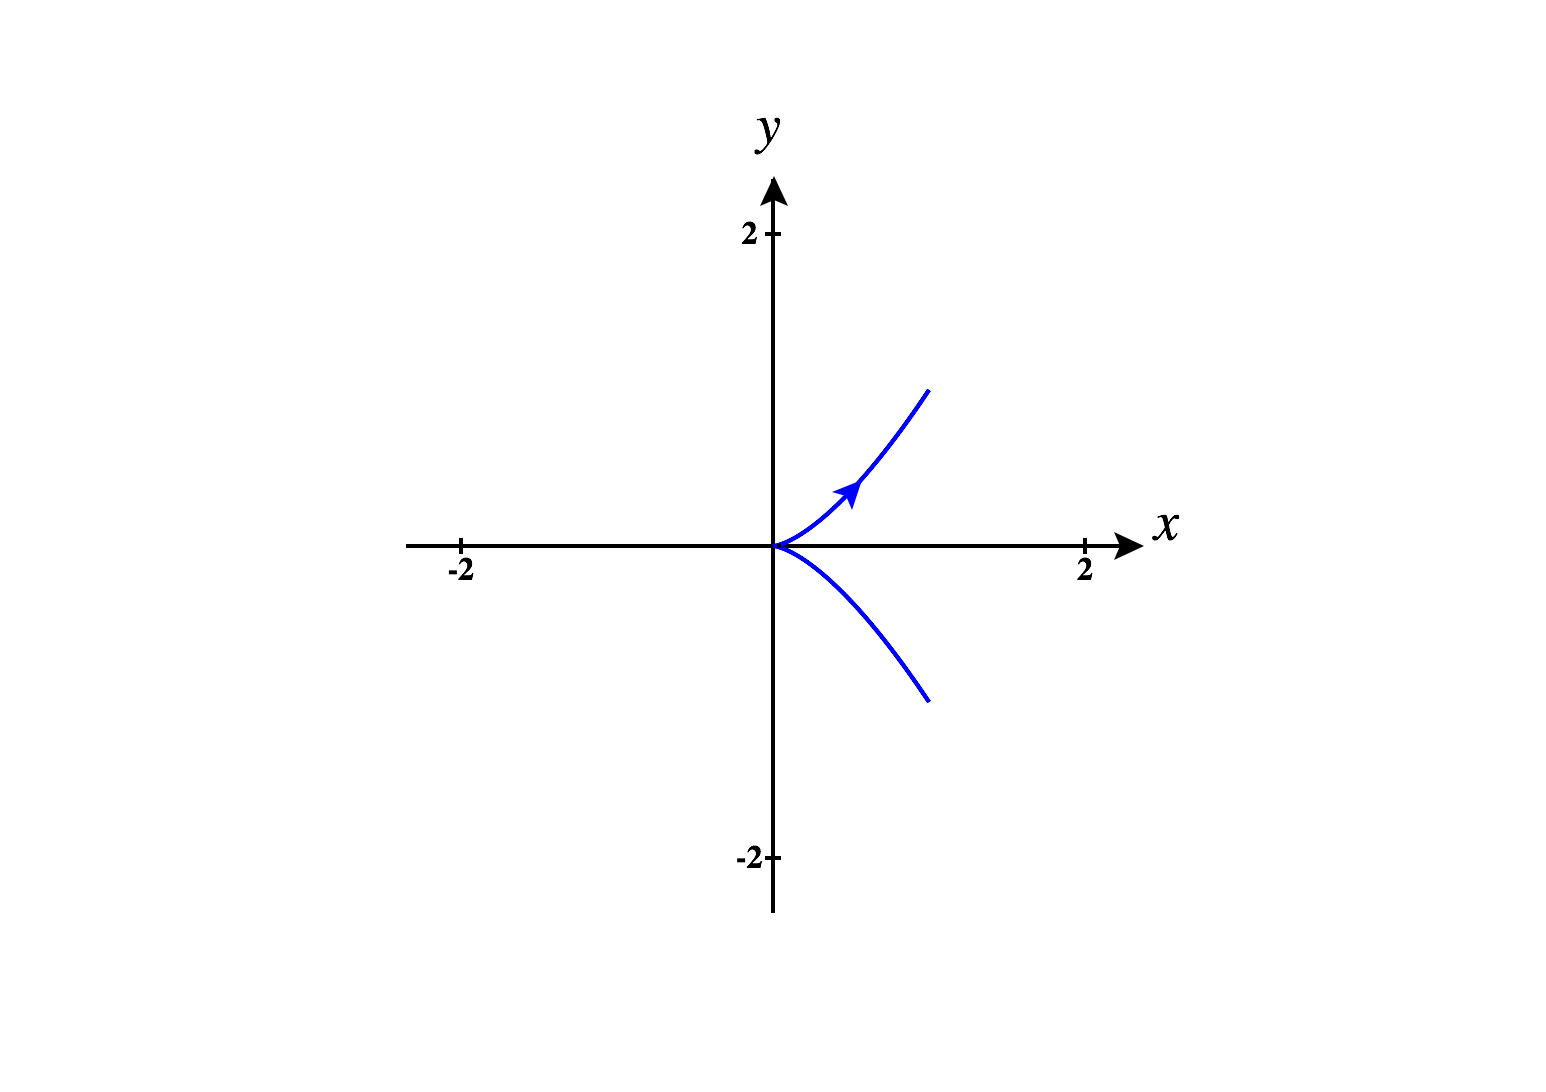
\includegraphics[width =\textwidth]{CalcPlot3D-cusp_correct}\end{image}}
\choice{\begin{image}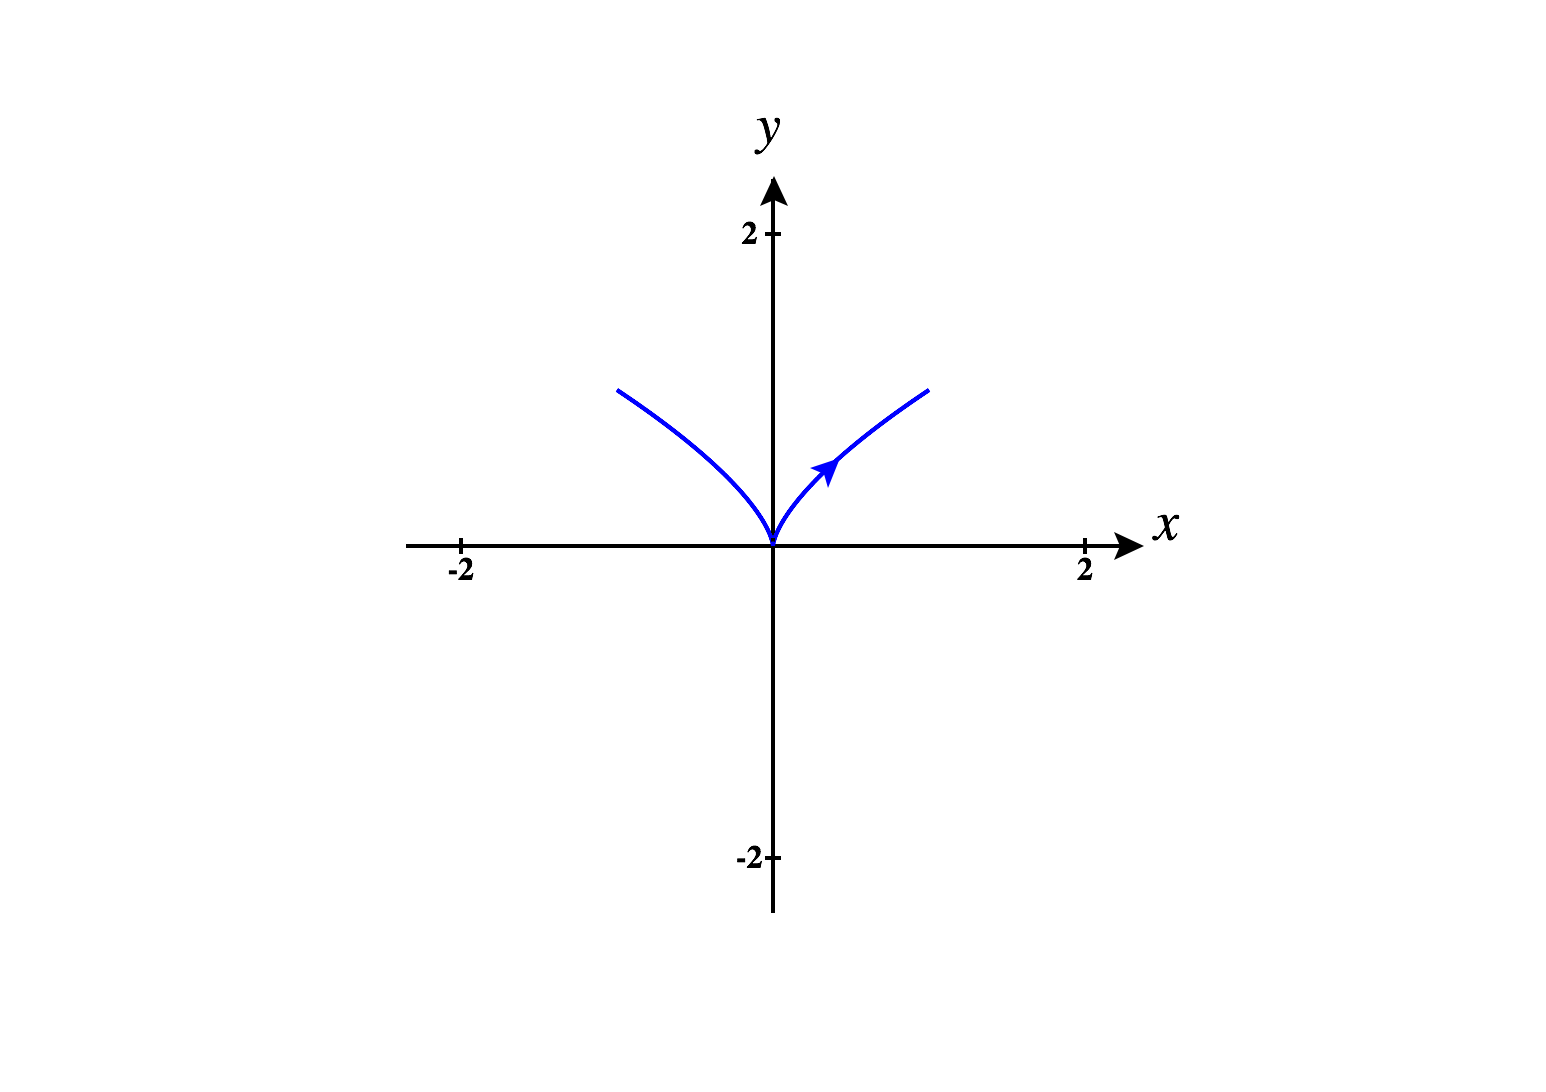
\includegraphics[width =\textwidth]{CalcPlot3D-cusp_incorrect1}\end{image}}
\choice{\begin{image}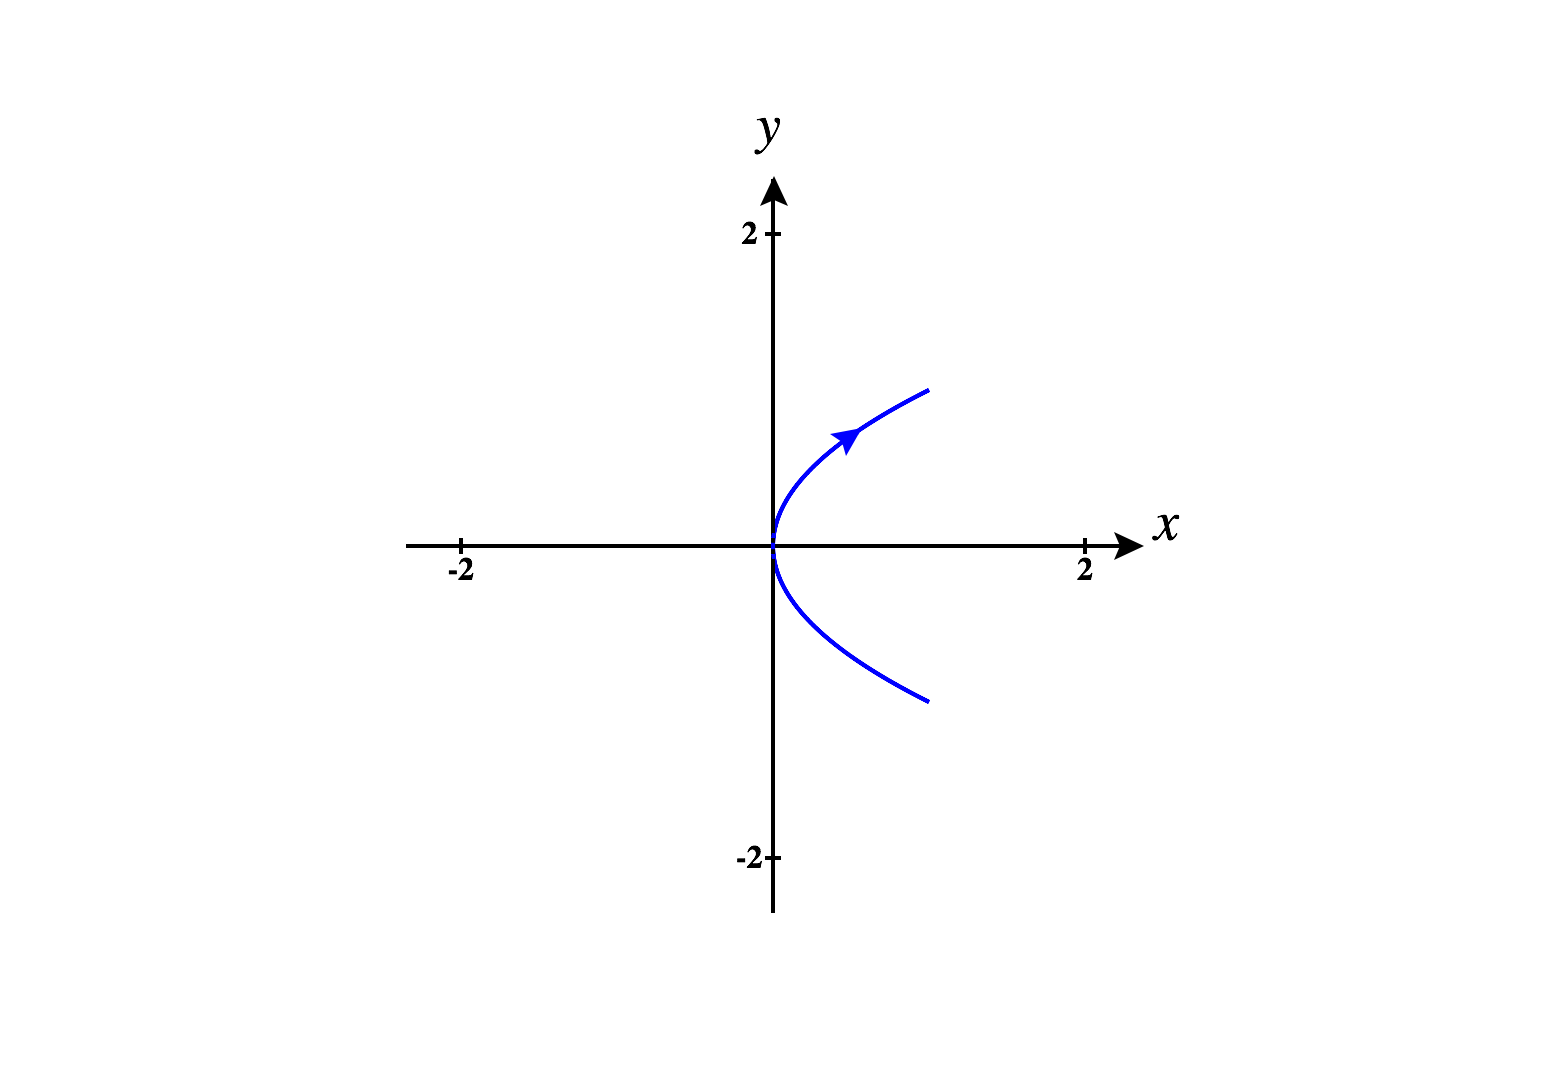
\includegraphics[width =\textwidth]{CalcPlot3D-cusp_incorrect2}\end{image}}
\choice{\begin{image}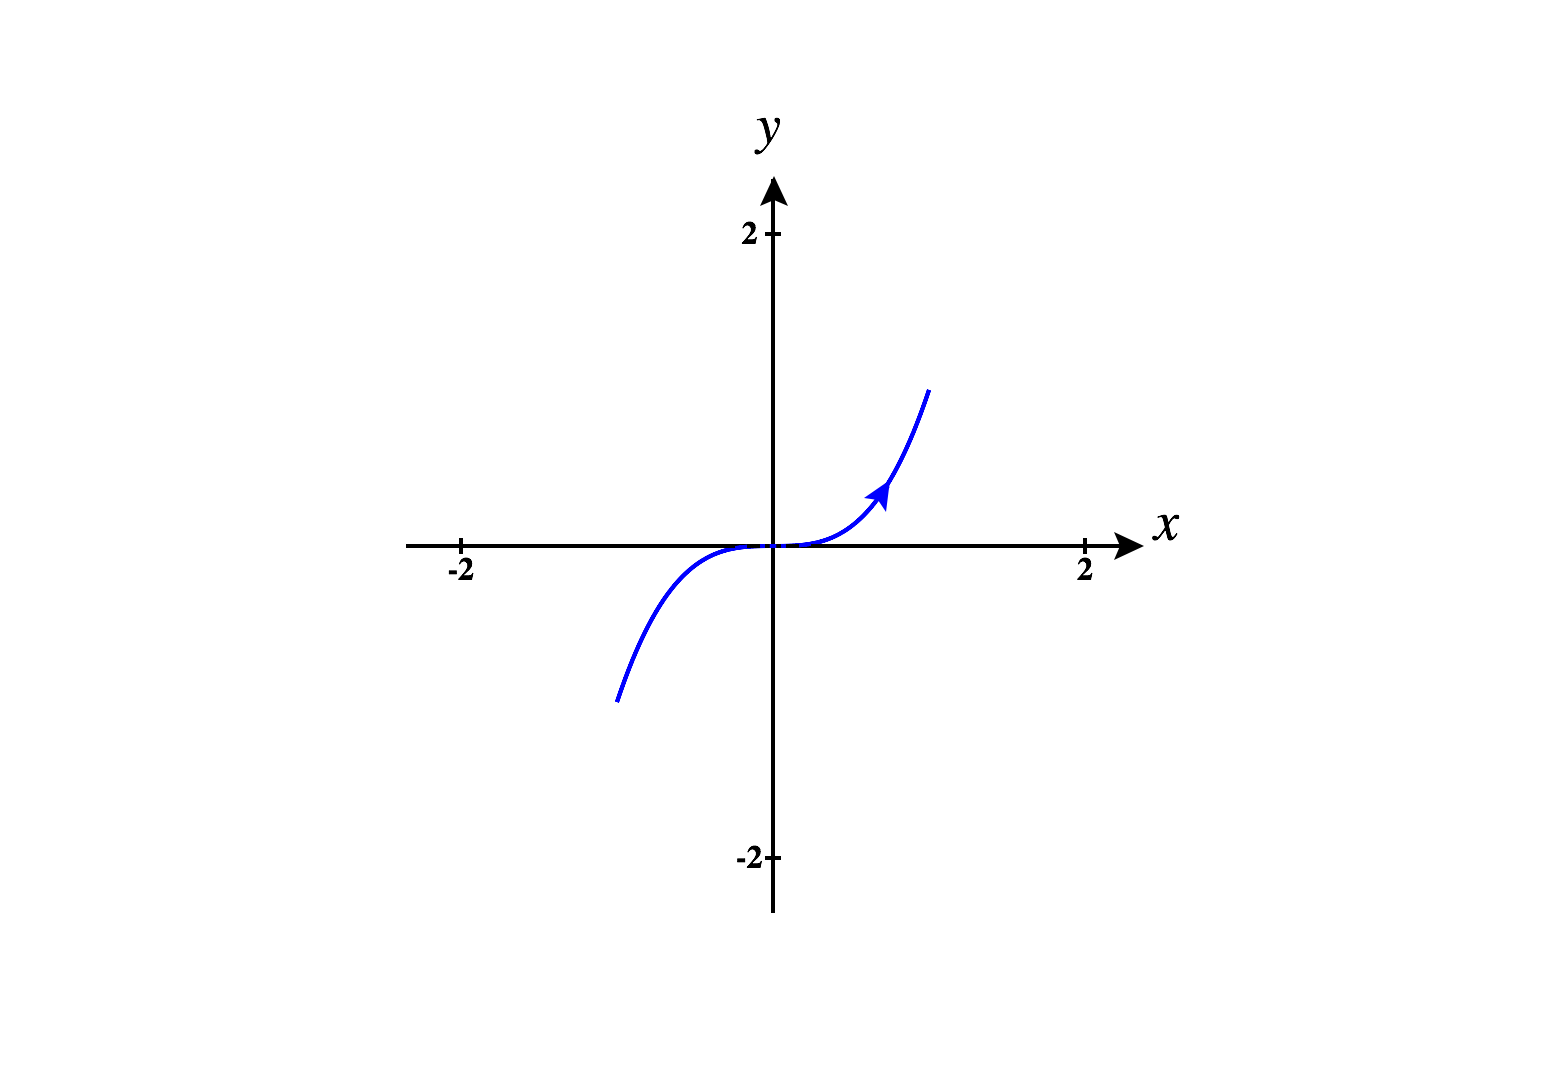
\includegraphics[width =\textwidth]{CalcPlot3D-cusp_incorrect3}\end{image}}
\choice{\begin{image}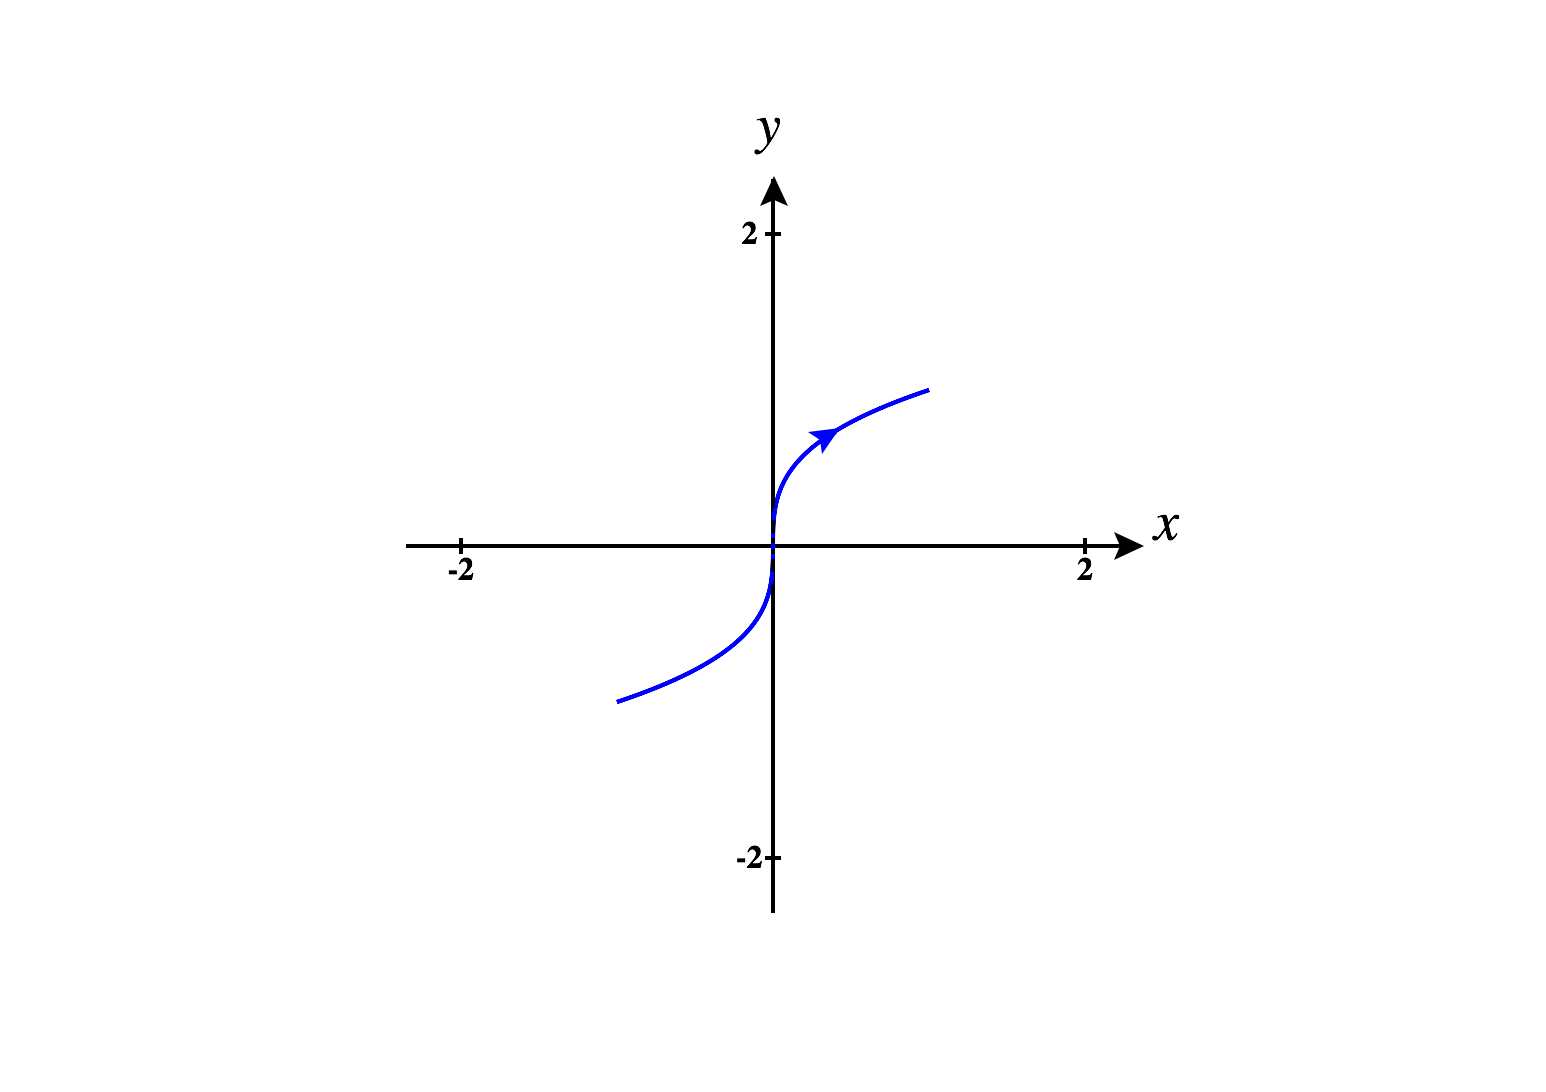
\includegraphics[width =\textwidth]{CalcPlot3D-cusp_incorrect4}\end{image}}
\end{multipleChoice}
\end{problem}

\begin{problem}
Consider the curve below.

\begin{image}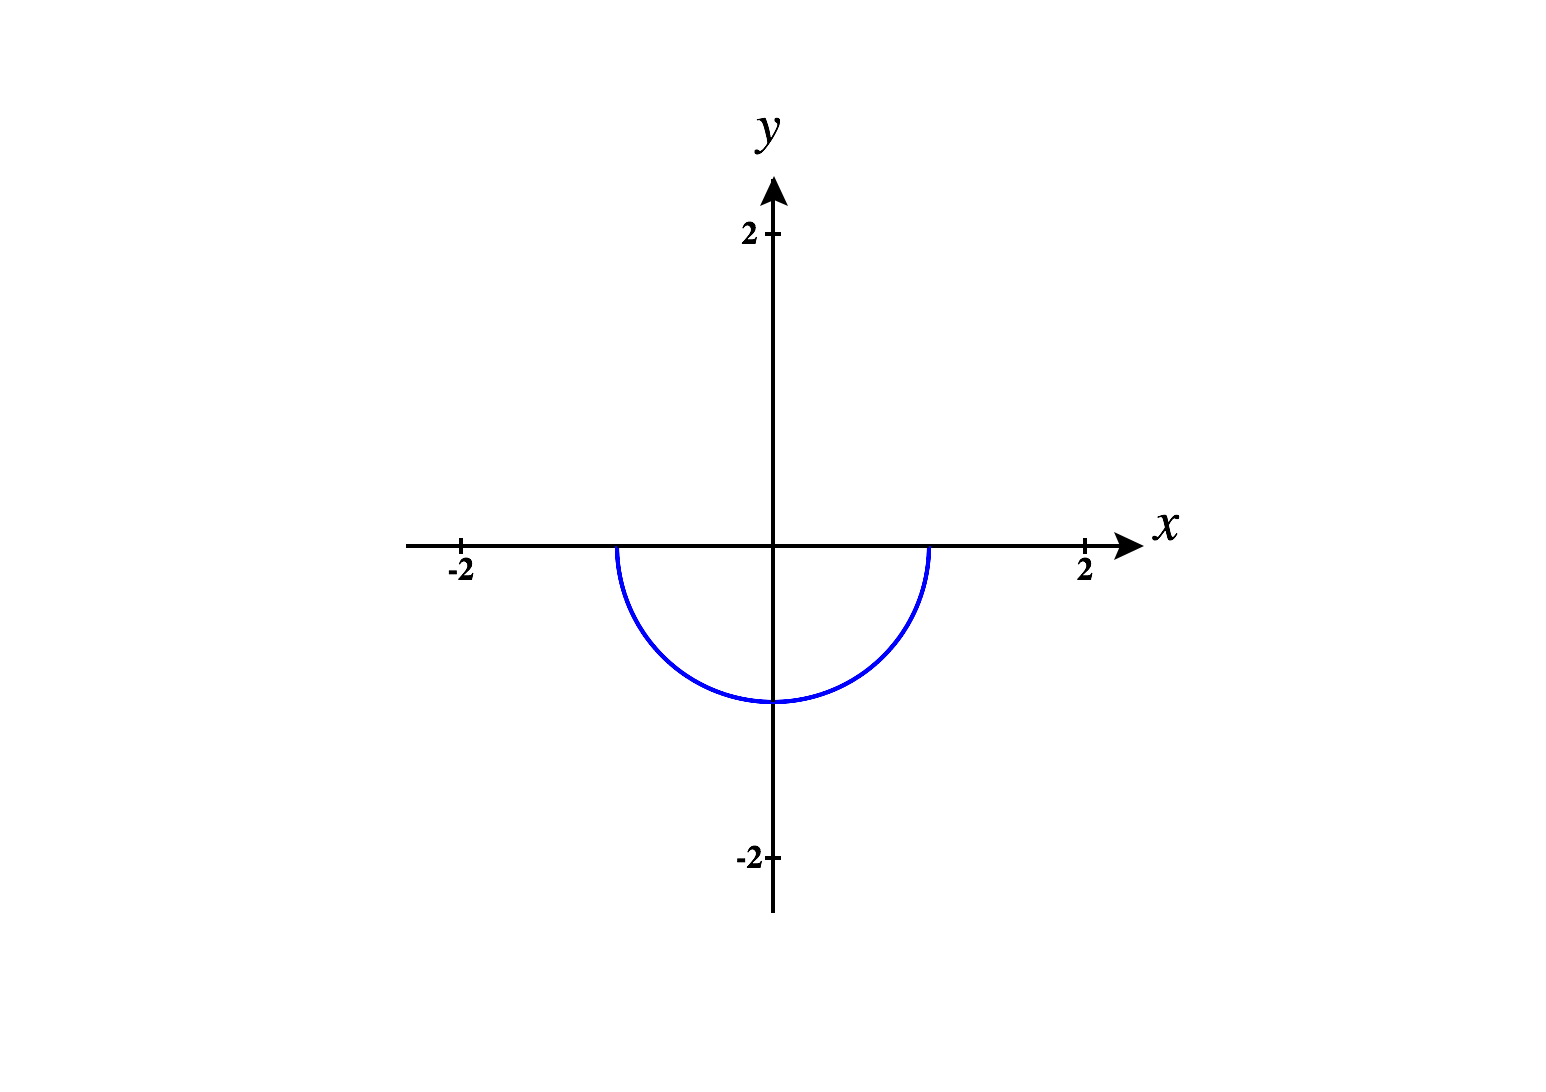
\includegraphics[width =\textwidth]{CalcPlot3D-half_circle}\end{image}

Which of the following are parametrizations for the curve? Select all that apply.
\begin{selectAll}
\choice{$\vec{x}(t) = (\cos t, \sin t)$, for $0\leq t\leq 2\pi$}
\choice{$\vec{x}(t) = (\sin t , \cos t)$, for $0\leq t\leq \pi$}
\choice[correct]{$\vec{x}(t) = (\cos t, -\sin t)$, for $0\leq t\leq \pi$}
\choice{$\vec{x}(t) = (-\cos t, \sin t)$, for $0\leq t\leq \pi$}
\choice[correct]{$\vec{x}(t) = (\sin t , \cos t)$, for $\pi/2\leq t\leq \pi/2$}
\choice[correct]{$\vec{x}(t) = (\cos t, \sin t)$, for $\pi\leq t\leq 2\pi$}
\choice{$\vec{x}(t) = (-\sqrt{1-t^2}, t)$ for $-1\leq t\leq 1$}
\choice{$\vec{x}(t) = (\sqrt{1-t^2}, t)$ for $0\leq t\leq 1$}
\choice[correct]{$\vec{x}(t) = (t,-\sqrt{1-t^2})$ for $-1\leq t\leq 1$}
\end{selectAll}
\end{problem}

\begin{problem}
Consider the curve below.

\begin{image}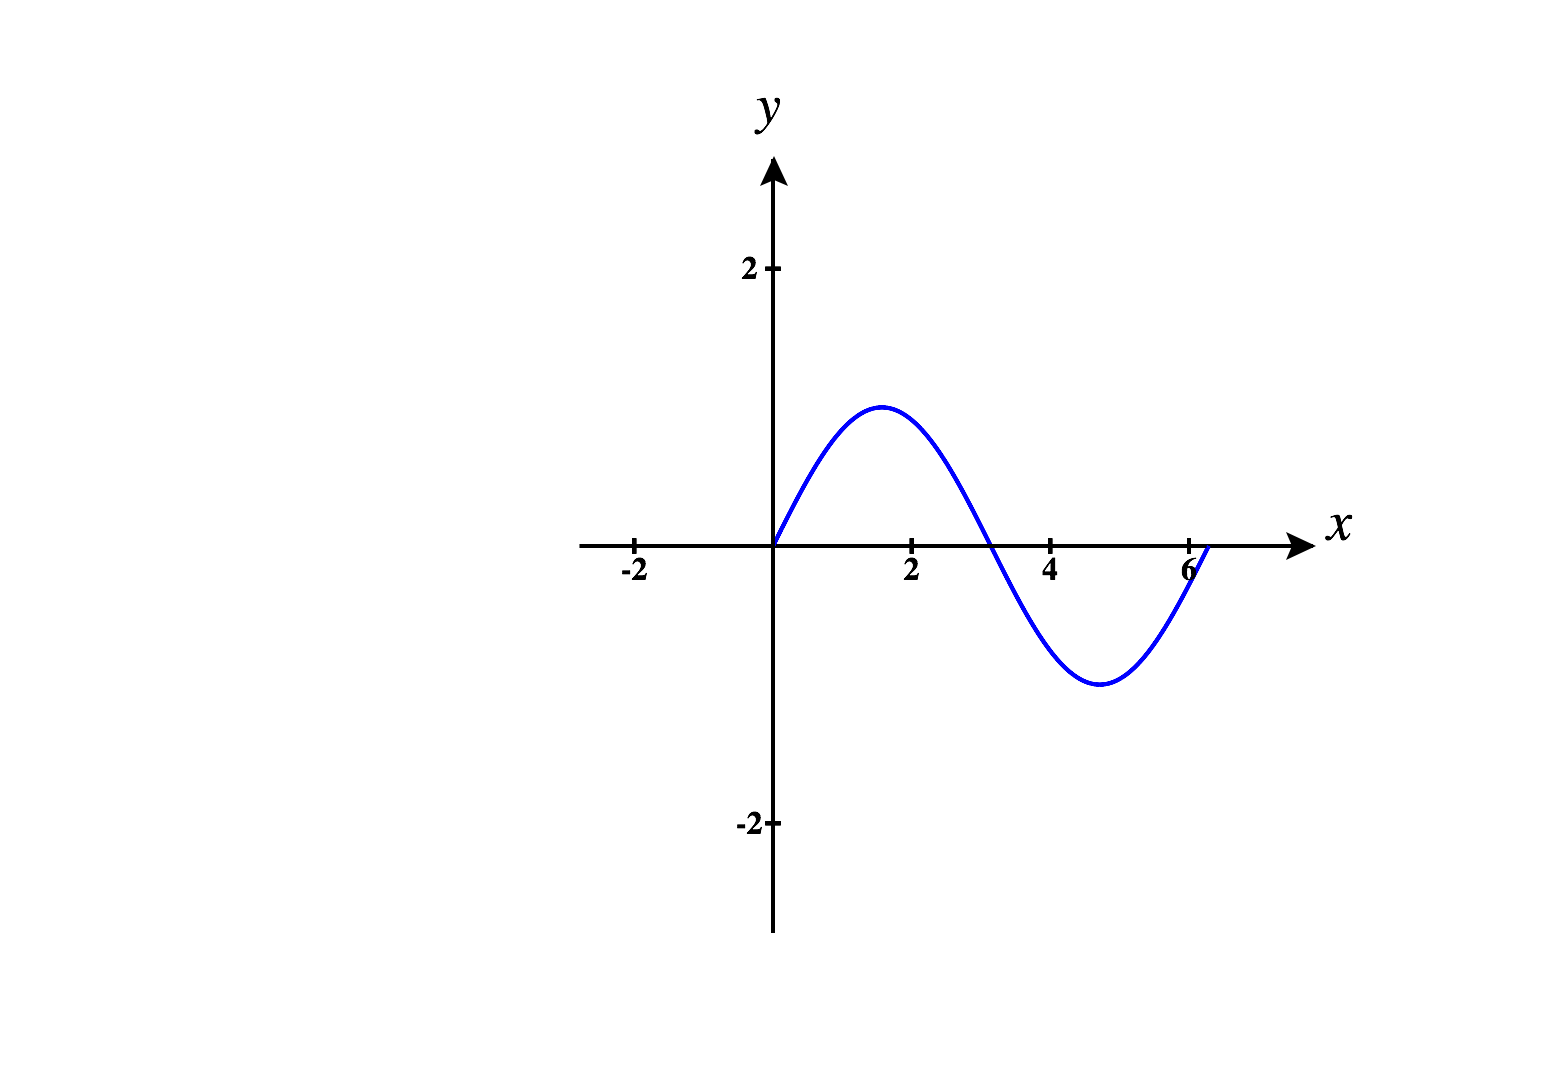
\includegraphics[width =\textwidth]{CalcPlot3D-sine_curve}\end{image}

Which of the following are parametrizations for the curve? Select all that apply.
\begin{selectAll}
\choice[correct]{$\vec{x}(t) = (t,\sin t)$ for $0\leq t\leq 2\pi$}
\choice{$\vec{x}(t) = (\arcsin t, t)$ for $-1\leq t\leq 1$}
\choice[correct]{$\vec{x}(t) = (2t^2,\sin (2t^2))$ for $-1\leq t\leq 1$}
\choice{$\vec{x}(t) = \left(t, \cos\left(\frac{\pi/2}(t-1)\right)\right)$ for $0\leq t\leq 2$}
\choice{$\vec{x}(t) = \left(\frac{\pi}{2}t, \cos\left(\frac{\pi/2}t\right)\right)$ for $0\leq t\leq 2$}
\choice{$\vec{x}(t) = \left(\frac{\pi}{2}t, \cos\left(\frac{\pi/2}(t-1)\right)\right)$ for $0\leq t\leq 2$}
\choice[correct]{$\vec{x}(t) = \left(\frac{\pi}{2}t, \cos\left(\frac{\pi/2}(t-1)\right)\right)$ for $0\leq t\leq 4$}
\end{selectAll}
\end{problem}

\begin{problem}
Consider the path $\vec{x}(t) = (3\cos(t), -2\sin(t))$, for $t\in\mathbb{R}$.

Compute the velocity of $\vec{x}$.
\[
\vec{v}(t) = \answer{(-3\sin(t), -2\cos(t))}
\]
Compute the speed of $\vec{x}$.
\[
\|\vec{x}'(t)\| = \answer{\sqrt{13}}
\]
Compute the acceleration of $\vec{x}$.
\[
\vec{a}(t) = \answer{(-3\cos(t), 2\cos(t))}
\]
\end{problem}

\begin{problem}
Two ants are running on the top of a table. Their paths are described by
\[
\vec{x}(t) = (t^2+1,2t-1)
\]
and
\[
\vec{y}(t) = (\sqrt{t+3}, t),
\]
with coordinates in inches, for $t\geq 0$ in seconds.

At what time do the ants collide?
\[
t = \answer{1}
\]

Where do the ants collide?
\[
(x,y) = \answer{(2,1)}
\]
\end{problem}

\begin{problem}
Consider the curve $\vec{x}(t) = (4t+2, 1-3t)$ for $t\in\mathbb{R}$.

Compute the velocity.
\[
\vec{v}(t) = \answer{(4,-3)}
\]

Compute the speed.
\[
\|\vec{x}'(t)\| = \answer{4}
\]
Compute the acceleration.
\[
\vec{a}(t) = \answer{(0,0)}
\]
\end{problem}

\begin{problem}
Consider the curve $\vec{x}(t) = (2\cos t, 5\sin t, t^2)$ for $t\in\mathbb{R}$.

Find the velocity.
\[
\vec{v}(t) = \answer{(-2\sin t, 5\cos t, 2t)}
\]
Find the velocity when $t = \pi$.
\[
\vec{v}(\pi) = \answer{(0,-5,2\pi)}
\]
Find a parametrization for the tangent line to $\vec{x}$ at the point where $t = \pi$, so that $L(0) = \vec{x}(\pi)$.
\[
L(t) = \answer{(-2,5,\pi^2) + t(0,-5,2\pi)}
\]
\end{problem}

\begin{problem}
Consider the curve $\vec{x}(t) = (t, t^2, t^3)$ for $t\in\mathbb{R}$.

Find the velocity.
\[
\vec{v}(t) = \answer{(1, 2t, 3t^2)}
\]
Find the velocity when $t = 2$.
\[
\vec{v}(\pi) = \answer{(1,4,12)}
\]
Find a parametrization for the tangent line to $\vec{x}$ at the point where $t = 2$, so that $L(0) = \vec{x}(2)$.
\[
L(t) = \answer{(2,4,8) + t(1,4,12)}
\]
\end{problem}

\begin{problem}
Consider the curve $\vec{x}(t) = (t, te^t, e^{t^2})$ for $t\in\mathbb{R}$.

Find the velocity.
\[
\vec{v}(t) = \answer{(1, e^t+te^t, 2te^{t^2})}
\]
Find the velocity when $t = 0$.
\[
\vec{v}(\pi) = \answer{(1,1,0)}
\]
Find a parametrization for the tangent line to $\vec{x}$ at the point where $t = 0$, so that $L(0) = \vec{x}(0)$.
\[
L(t) = \answer{(0,0,1) + t(1,1,0)}
\]
\end{problem}

\section*{Written Problems}
\begin{problem}
\begin{enumerate}
\item Graph the surface $z^2 = x^2 +y^2$ and the curve $\vec{x}(t) = (t\cos(t), t\sin(t), t)$ for $-5\leq t\leq 5$.
\item Verify algebraically that the curve lies on the surface.
\end{enumerate}
\end{problem}

\begin{problem}
Prove the following product rule for cross products.

Let $\vec{x}$ and $\vec{y}$ be paths in $\mathbb{R}^3$, then 
\[
(\vec{x}\times\vec{y})'(t) = \vec{x}'(t)\times\vec{y}(t) + \vec{x}\times\vec{y}'(t),
\]
for $t$ such that $x'(t)$ and $y'(t)$ exist.
\end{problem}

\section*{Professional Problem}

\begin{problem}
\begin{enumerate}
\item Let $\vec{x}(t)$ be a curve lying on a sphere in $\mathbb{R}^n$ of radius $C$. Prove that $\vec{x}(t)$ and $\vec{x}'(t)$ are perpendicular. 
\item For the curve $\vec{x}(t) = (\cos(t), \sin^2(t), \cos(t)\sin(t))$, verify computationally that $\vec{x}(t)$ lies on the sphere, and that $\vec{x}'(t)$ is perpendicular to $\vec{x}(t)$.
\end{enumerate}
\end{problem}



\end{document}